\chapter{System Usage}
This section documents the steps required for correct usage of the data acquisition system.

\section{Integration}
The main data acquisition system should be integrated into the flight test vehicle near the vehicle's center of gravity.\nomenclature[A]{CG}{Center of gravity} The system should have one of its principal axes lined up roughly parallel to the vehicle's longitudinal axis. Servos should be connected to both the main board and the aircraft's receiver using a y-splitter with 2 male and one female connectors. If applicable, the servos should be connected according to the Table \ref{table:servoSetup}.
\begin{table}[ht]
\caption{Air Data System Setup} % title of Table
\centering % used for centering table
\begin{tabular}{c c} % centered columns (4 columns)
\hline\hline %inserts double horizontal lines
 Servo & PWM Pinout\\
\hline % inserts single horizontal line
Throttle & D37\\
Elevator & D38\\
Rudder & D39\\ 
Aileron (1/2) & D40\\
Aileron (2/2) & D41\\
Gear & D42\\
Auxiliary (1/2)& D43\\
Auxiliary (2/2)& D44\\
\hline
\end{tabular}
\label{table:servoSetup}
\end{table}

If the additional digital pinouts are being use for measuring servo signals, the ``+V'' jumper should not have a jumper on it. If using the digital pinouts to run digital sensors or command servos, place the jumper on the appropriate voltage level setting.

The pressure board can be placed anywhere in the vehicle, as long as it can be connected to the main board. The pressure sensors should be attached to the five-hole probe as follows:

\begin{table}[ht]
\caption{Air Data System Setup} % title of Table
\centering % used for centering table
\begin{tabular}{c c c c} % centered columns (4 columns)
\hline\hline %inserts double horizontal lines
 Pressure Sensor & Port A & Port B & Measurement\\
\hline % inserts single horizontal line
0 & Tube 4 & Tube 5 & $\beta$ \\
1 & Tube 1 & Tube 6 & $q_{\infty}$\\
2 & Tube 2 & Tube 3 & $\alpha$\\ 
3 & n/a & Tube 6 & $P_S$\\
\nomenclature[A]{$P_S$}{Static pressure}\\
\hline
\end{tabular}
\label{table:airDataSetup}
\end{table}
Port A and Port B refer to the ports as labeled in Figure \ref{fig:pressureLabels}, and the tube number refers to the five-hole probe tubes. These tube numbers increase as the tube legth decreases: Tube 1 refers to the longest tube, Tube 6 refers to the shortest tube.

\begin{figure}[H]
  \centering
    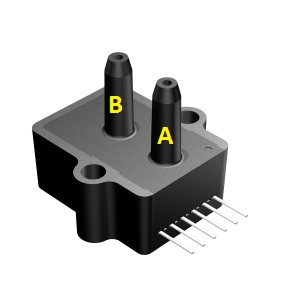
\includegraphics[width=0.5\textwidth]{figures/allsensorsPressureLabeled.jpg}
      \caption{Port Description for Pressure Sensors} \label{fig:pressureLabels}
\end{figure}

The pressure tubing and temperature sensor line should be routed together to the air data boom and secured for flight. The temperature sensor's wiring is a standard servo extension. The air data boom's accelerometer wiring is a standard RJ-25 \textit{patch} cable and should be routed in a separate bundle, as it will be removed before flight.

The air data boom itself should be integrated as far from aerodynamic effects as possible. For this thesis, the boom was mounted roughly one chord length in front of the leading edge of the wing and approximately halfway down the wing span. Other mounting locations could include out the aircraft's nose for a pusher vehicle, or on the vertical tail. The aluminum block accepts a 0.25" carbon fiber tube as it's mounting interface, and this tube should be mounted roughly in-line with the airflow angle expected during flight. The temperature sensor can be taped to the tube.

\section{Pre-flight Procedure}
\label{sect:preFlightProc}
The pre-flight procedure in this section must be completed in addition to all preparation listed in Section \ref{sect:flightTestDocs}.

\begin{enumerate}
\item With the transmitter turned on, power on the receiver.
\item Plug in the micro-USB cable into the main data acquisition board.
\item Ensure the micro-SD card is empty and formatted as FAT32, then insert it into the main data acquisition board.
\item Plug in the main data acquisition system's battery pack.
\item Plug the pressure sensor board into the main data acquisition board.
\item Plug in the air data system's RJ-25
\item Upload the calibration routine to the main board, and follow the prompts to calibrate the gyroscope, accelerometer, and magnetometers.
\item Place a wind blocker (Daisy/Solo cups work) over the five-hole probe and calibrate the pressure sensors, using the calibration routine.
\item Calibrate the air data system's orientation using the calibration routine.
\item Load the main data acquisition script onto the main data acquisition board.
\item Turn on serial output and check that all sensors are functioning properly.
\item Initialize the micro-SD card.
\item Turn off serial output.
\item Turn on data logging and verify the system is saving data.
\item Remove the micro-USB cable and the air data system's RJ-25 cable.
\end{enumerate}
Talk about the pre-flight calibration process:
air data boom orientation
pressure offset calibration
accel/gyro calibration
magnetometer calibration


After the flight is complete, a second round of zero offset calibration data should be acquired. This set ensures that any drift that occurred during the flight is accounted for. Repeat the steps outlined in Section \ref{preflightZeroCalib}.

\section{Flight test plan}
Yo bro, glide around for a while. change speeds and stuff.

\section{Post-flight}
Let's talk about how to use that sweet GUI of yours.

\section{Software protocol}
List of commands available for the mainScript and calib scripts, along with how they work.